\subsection{Descarga e instalación de Python}
A continuación, te dejaré un video para aprender de manera más práctica y visual, tienes que seguir los pasos que se mencionan: \href{https://www.youtube.com/watch?v=cmItObuFBuA}{Tutorial}

\begin{figure}[h]
    \centering
    \scalebox{0.35}{
    
\includegraphics{Imagenes/instalacion1.png}
    }
  \end{figure}

Siguiendo con algo más teórico, para comenzar a programar en Python, primero necesitas instalar Python en tu sistema. Puedes hacerlo siguiendo estos pasos:

\begin{itemize}
    \item[a. ]Descarga Python: Visita el sitio web oficial de Python en python.org y descarga la última versión de Python. Asegúrate de elegir la versión más reciente y compatible con tu sistema operativo (Windows, macOS, o Linux).
    \begin{figure}[h]
        \centering
        \scalebox{0.35}{
        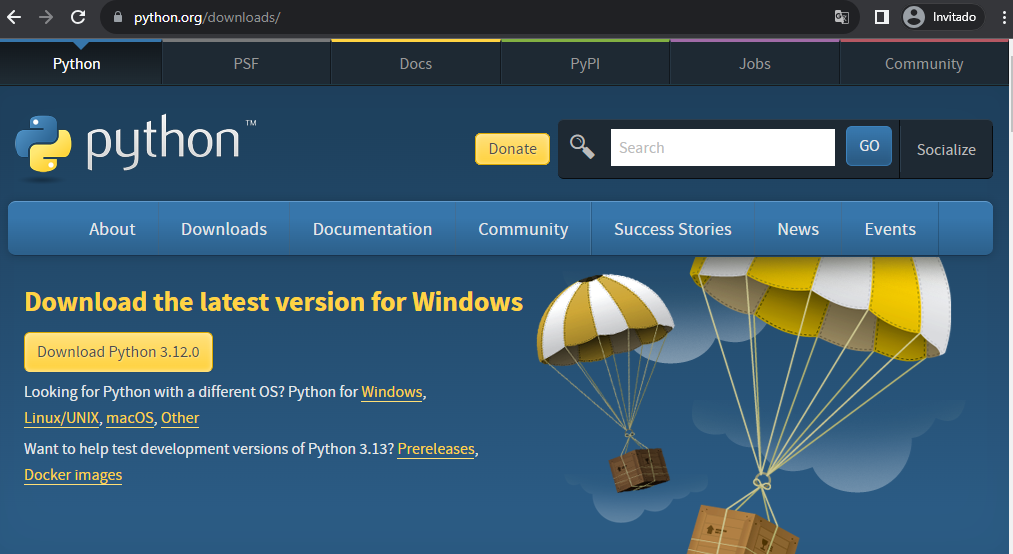
\includegraphics{Imagenes/instalacion2.png}
        }
      \end{figure}
    
    \item[b. ]Instalación en Windows: Ejecuta el archivo descargado y sigue las instrucciones del instalador. Asegúrate de marcar la opción ``Agregar Python al PATH'' durante la instalación.
    \begin{figure}[h]
        \centering
        \scalebox{0.35}{
        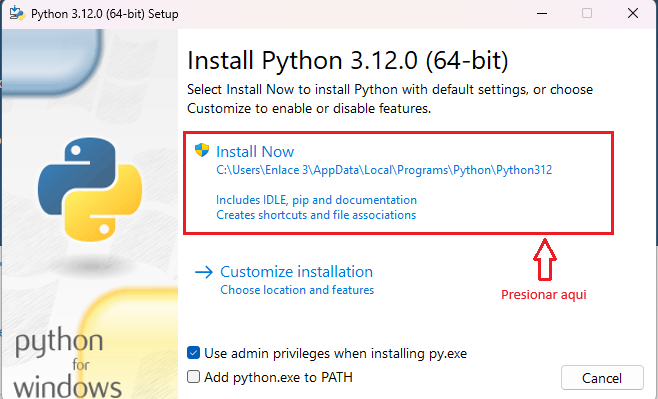
\includegraphics{Imagenes/instalacion3.png}
        }
      \end{figure}
\end{itemize}

\subsection{Configuración del entorno de desarrollo}
Puedes escribir y ejecutar código Python en un entorno de desarrollo integrado (IDE) o simplemente en un editor de texto. Algunas opciones populares para IDEs incluyen:\\

Elige el IDE o editor de tu preferencia y configúralo.
\begin{itemize}
    \item IDLE: es un programa que te ayuda a escribir y ejecutar código en Python. Es útil para principiantes porque combina un espacio para escribir código y un lugar para ver los resultados, lo que facilita aprender y probar cosas nuevas en Python. Tutorial de Cómo instalar Python y usar la herramienta IDLE: 
    \href{https://www.youtube.com/watch?v=F9eM_VoKGJQ}{Revisa este link para más ayuda}
    \begin{figure}[h]
        \centering
        \scalebox{0.35}{
        
\includegraphics{Imagenes/instalacion4.png}
        }
      \end{figure}

    \item PyCharm: Un IDE muy popular y potente para Python. Tutorial de Como instalar y configurar Pycharm:
    \href{https://www.youtube.com/watch?v=wxdafAAzIWo }{Revisa este link para más ayuda}
    \begin{figure}[h]
        \centering
        \scalebox{0.35}{
        
\includegraphics{Imagenes/instalacion5.png}
        }
      \end{figure}

    \item Visual Studio Code (VSCode): Un editor de código que es altamente configurable y ampliamente utilizado para Python. Tutorial de como instalar y Configurar Visual Studio Code:
    \href{https://www.youtube.com/watch?v=X_Z7d04x9-E}{Revisa este link para más ayuda}
    \begin{figure}[h]
        \centering
        \scalebox{0.35}{
        
\includegraphics{Imagenes/instalacion6.png}
        }
      \end{figure}
\end{itemize}

\subsection{Tu primer programa en python}

Una vez que hayas instalado Python y configurado tu entorno de desarrollo, puedes comenzar a escribir código Python. Aquí tienes un ejemplo de un programa Python simple:
\begin{figure}[h]
    \centering
    \scalebox{0.35}{
    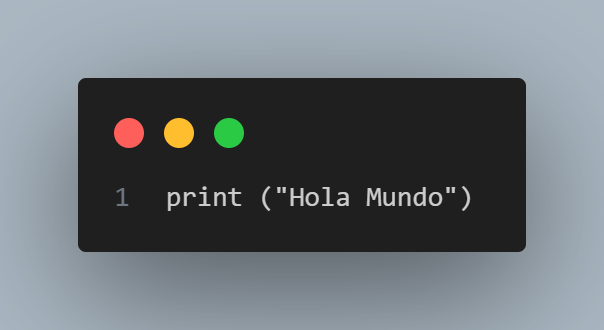
\includegraphics{Imagenes/instalacion7.png}
    }
  \end{figure}
Para ejecutar el código, guárdalo en un archivo con extensión ``.py'' (por ejemplo, ``mi\_programa.py'') y ejecútalo desde la línea de comandos o desde tu IDE.

